\documentclass[11pt, oneside]{article} 
\usepackage{geometry}
\geometry{letterpaper} 
\usepackage{graphicx}
	
\usepackage{amssymb}
\usepackage{amsmath}
\usepackage{parskip}
\usepackage{color}
\usepackage{hyperref}

\graphicspath{{/Users/telliott/Github/precalculus/fig/}}
% \begin{center} \includegraphics [scale=0.4] {gauss3.png} \end{center}

\title{Right triangles}
\date{}

\begin{document}
\maketitle
\Large

The main result we are headed for is the Pythagorean Theorem.  Before we get there, however, it is worthwhile to continue our development of basic geometry with a discussion about right angles and right triangles.  

A right triangle is a triangle containing one right angle.  Right angles (and right triangles) are special.  We saw previously that the definition of a right angle is that two of them add up to one straight line or $180$ degrees.  

Since we proved that the sum of the three angles in any triangle is equal to one straight line, by extension, the sum of angles in any triangle is also equal to two right angles.

In the figure below, the angle at vertex $P$ is a right angle.  It is common to mark a right angle with a little square, as shown, but these are a pain to draw, so I will often not do that.  The side opposite $P$, namely $c$, is the \emph{hypotenuse}.

\begin{center} 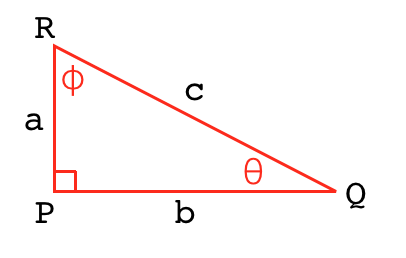
\includegraphics [scale=0.35] {right_triangle.png} \end{center}

Since the sum of angles in a triangle is equal to two right angles, the sum of the angles $\theta$ and $\phi$ above is also equal to one right angle, or 90 degrees.  

Angles $\theta$ and $\phi$ are said to be \emph{complementary}.  This fact is often exploited in proofs.

\textcolor{red}{
$\bullet$ \ the two smaller angles in a right triangle add to 90 degrees.}

\subsection*{hypotenuse-leg (HL)}
 
For two right-triangles, if one hypotenuse is equal to the other, and also one set of legs equal, the two triangles are congruent.

\begin{center} 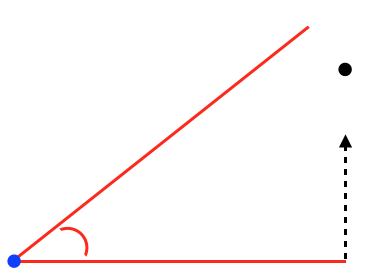
\includegraphics [scale=0.4] {hyp_side_cong.png} \end{center}

In the figure, imagine the hypotenuse swinging on the hinge of its vertex with the horizontal base.  There is only one angle where it will terminate on the vertical side with the correct length.  This determines the angle between the known sides, or alternatively, the length of the third side. 

We really have SSA (which we said doesn't work always).  However, it does work for right triangles.   

Previously we showed this figure:

\begin{center} 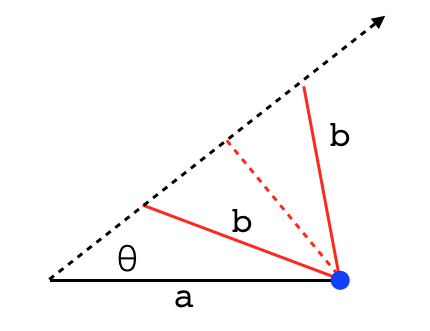
\includegraphics [scale=0.4] {angle_side_side.png} \end{center}

and we said that in the special case where $b$ meets the opposing side in a right angle, that SSA is enough to prove congruence.  Call it HL to be safe, but it does work.

Other named methods of proof for right triangles can be found in books, but these do not add anything because they are exactly equivalent to methods we already know:

$\circ$ Leg-Leg, the two legs flank the right angle (SAS).

$\circ$ Hypotenuse-Acute angle (AAS).

$\circ$ Leg-Acute angle (ASA).

\subsection*{altitudes}

\begin{center} 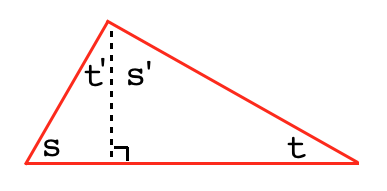
\includegraphics [scale=0.5] {complementary.png} \end{center}

In the large right triangle above, we know that
\[ s + t = 90 \]
When we draw the perpendicular to the hypotenuse that goes through the upper vertex, that is an \emph{altitude} of the triangle.  Because of the right angle, we obtain two smaller right triangles.  Thus
\[ s + t' = 90 \]
\[ s' + t = 90 \]
Hence
\[ s + t = s + t' \]
\[ t = t' \]
and similarly for $s$ and $s'$.

\subsection*{angle bisectors}

We want to prove a theorem about angle bisectors, as well as its converse.  Before we do that, we need three theorems about right triangles.

$\bullet$ \ In any right triangle, the right angle is larger than either of the other two angles.

Proof.

Suppose $\alpha$ and $\beta$ are complementary angles in a right triangle,  Then $\alpha + \beta$ is equal to one right angle.  But the measure of both angles is non-zero.  Therefore $\alpha < 90$ and the same for $\beta$.

$\square$

$\bullet$ \ In any right triangle, the hypotenuse is longer than either side.

Proof.

By the previous theorem, the right angle is the largest angle in a right triangle.

By (Euclid \hyperref[sec:Euclid1]{\textbf{Prop $I.18$}} in the next chapter):  in any triangle, a greater side is opposite a greater angle.  

$\square$

$\bullet$ \ The distance from a point to a line is least at the point where the new line segment makes a right angle with the line.

\begin{center} 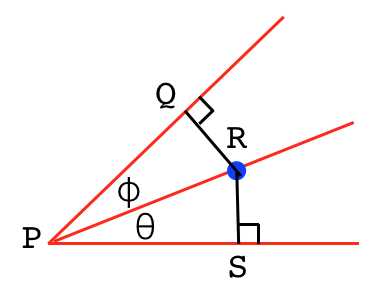
\includegraphics [scale=0.4] {angle_bisector2.png} \end{center}

Proof.

Consider $QR$.  Any other line segment forms a right triangle with $QR$, where that line segment is the hypotenuse.  By the previous theorem, $QR$ must be shorter.

So then:

$\bullet$ \ Any point on the bisector of an angle is equidistant from the sides at the point of closest approach.

\begin{center} 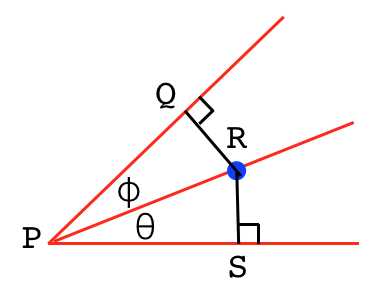
\includegraphics [scale=0.4] {angle_bisector2.png} \end{center}

We simply draw the vertical line $RS$.  The resulting triangle is congruent to $\triangle PQR$ by AAS.  Therefore, $QR = RS$.

$\square$

$\bullet$ \ If a point is equidistant from the sides of an angle, then it lies on the angle bisector.

Proof.

Use SAS to prove the same congruence as in the previous theorem.  Then, $\angle \theta = \angle \phi$.


\subsection*{stacked triangles}

\begin{center} 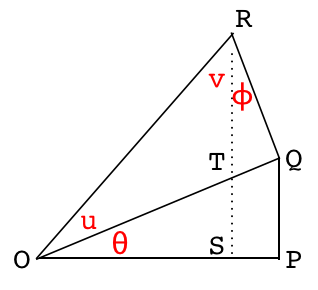
\includegraphics [scale=0.5] {angle_bisector_r4.png} \end{center}

Suppose we are given that $\angle OPQ$ and $\angle OQR$ are right angles.  We draw the altitude $RS$ and observe that the angle at vertex $S$ is a right angle.  

Therefore, in triangle $ORS$, the sum $\theta + u + v$ is equal to one right angle.  At the same time, in triangle $OQR$, the sum $u + v + \phi$ is also equal to one right angle.  Therefore
\[ \theta = \phi \]

Further, $\triangle QRT$ and $\triangle OPQ$ are similar triangles.

\subsection*{angle bisector}

\label{sec:angle_bisector}

With that background, we now consider a classic problem:  the ratio of sides when there is an angle bisector.
\begin{center} 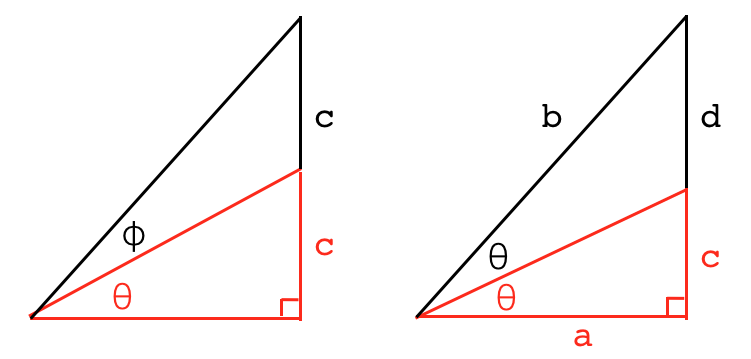
\includegraphics [scale=0.4] {angle_bisector_r1.png} \end{center}
Suppose we are given that the large triangle is a right triangle.  

We draw a line joining the vertex on the left with the side opposite. 

This line could in general be drawn anywhere, however two interesting cases are when  the side opposite is bisected (left panel), or when the angle at the left is bisected (right panel).  These two cases are not the same.  In the first $\phi \ne \theta$ and in the second, $c \ne d$.

Suppose we choose the second possibility, equal angles.  We are in a position to prove an important theorem.

\subsection*{angle bisector theorem}

With reference to the two figures above, we are to prove that
\[ \frac{d}{b} = \frac{c}{a} \]

$\bullet$ \ The sides and bases are in proportion for a right triangle with bisected angle.

Proof.

Draw an altitude for the upper of the two small triangles, meeting the side of length $b$.

\begin{center} 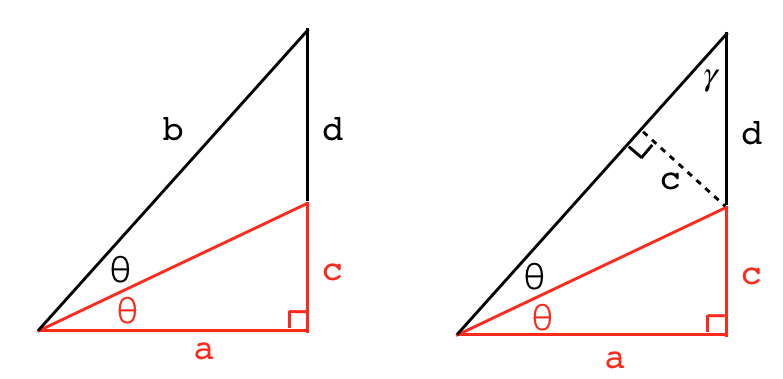
\includegraphics [scale=0.4] {angle_bisector_r2.png} \end{center}

The red triangle and the one directly above it are congruent (right panel).  They share a side (the hypotenuse of each), and they are right triangles with the same smaller angle $\gamma$.  Therefore, the altitude we just drew has length $c$.

The small triangle with sides $c$ and $d$ (at the top) is similar to the original large triangle.  The reason is that they are both right triangles containing the smaller angle $\gamma$.

By similar triangles, we form equal ratios of the angle opposite $\gamma$ to the hypotenuse:

\[ \frac{a}{b} = \frac{c}{d} \]

This is rearranged simply to give
\[ \frac{d}{b} = \frac{c}{a} \]
which is what we were asked to prove.

The result can be pushed a little further:
\[ \frac{a}{b} = \frac{c}{d} \]
Here's the key point
\[ \frac{a + b}{b} = \frac{c + d}{d} \]
\[ \frac{a + b}{c + d} = \frac{b}{d} = \frac{a}{c} \]

$\square$

\begin{center} 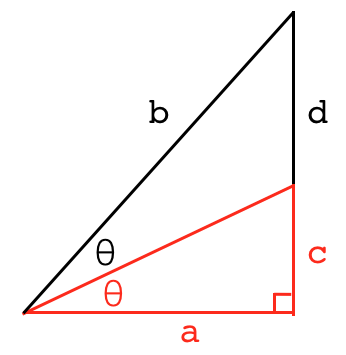
\includegraphics [scale=0.4] {angle_bisector_r5.png} \end{center}

which is a surprising result and becomes important later in looking at Archimedes method for approximating the value of $\pi$.
 
\end{document}